\section{Statistical Models for Epidemiological Rates}
\label{theory-rate_model}

The key to connecting the systems dynamics model from
Chapter~\ref{theory-system_dynamics} to the evidence base collected
through systematic review is the \emph{rate model}.  This is a
statistical model, which has its core features defined by its
likelihood function.  Here a likelihood function is a 
probability density function that assigns a value for the likelihood
of every possible rate value and uncertainty for a given parameter
values.  An examples will make this clearer, and for this I direct
your attention to the meta-analysis of
population prevalence on Schizophrenia in Western European Males in
2000.  The forest plot in
Figure~\ref{fig:theory-rate_model-schiz_forest} shows the results of
combining << TK >> studies using << TK >> different rate models.
As the figure demonstrates, the choice of rate model can have a huge effect
on the estimated uncertainty, and can have a noticable effect on the estimated
median as well. In what follows, I will develop a collection of rate models, starting with the
simplest and slowing adding complexity, while identifying the benefits
and drawbacks of each.  The models to come, in order, are the binomial model, the
beta-binomial model, the poisson model, the negative binomial model,
and several variants of the normal model.

\begin{figure}
\begin{center}
\includegraphics[width=\textwidth]{schiz_forest_plot.png}
\end{center}
\caption{Forest plot summarizing TK alternative models for
  meta-analysis of schizophrenia prevalence for Western European Males
  in TK.  The population prevalence mean estimated by the models ranges from
  TK to TK, and the width of the $95\%$ HPD interval of the
  population prevalence estimated by the models ranges from TK
  to TK.}
\label{fig:theory-rate_model-schiz_forest}
\end{figure}

\subsection{Binomial Model}
Conceptually, the simplest model for rate data if built from the
Binomial random variable, which follows the probability distribution
\[
\Pr[X=k\given n,\pi] = \binom{n}{k}\pi^n(1-\pi)^{n-k}
\]
I've used greek to emphasize that $\pi$ is the parameter, while $n$
and $k$ are data.

Although this equation may appear opaque, the intuition behind it is
simple: $n$ individuals were tested for a disease, and $k$ tested
positive. The formula then follows from the assumption that each
individual tests positive with probability $\pi$, and all the
knowing about the test results of any subset of individuals gives me
no information about what the test results the others will be
(these events are ``independent'').

This distribution inspires a computationally tractable and
theoretically appealing rate model for a observed population rate of
$r$ from a population of size $n$:
\[
p(p,n\given \pi) \propto \pi^{nr}(1-\pi)^{n(1-r)}.
\]
Note that it is not necessary to include the term $\binom{n}{nr}$,
because this does not depend on the model parameter $\pi$. There is a
constant of proportionality, which is necessary to make this rate
model truely a probability density function for any $\pi$, but happily
I will never need to use this, and I have use the ``proportional to''
symbol $\propto$ instead of equality to emphsize this fact.

The funnel plot in Figure~\ref{fig:theory-rate_model-binom_funnel}
shows the predictive distribution of this rate model for $\pi=<<
rate_model.pi_binomial_funnel >>$.  It also shows the potential
problem with this approach: the data, as gathered from systematic
literature review are much more dispersed than this distribution
predicts.

\begin{figure}[ht]
\begin{center}
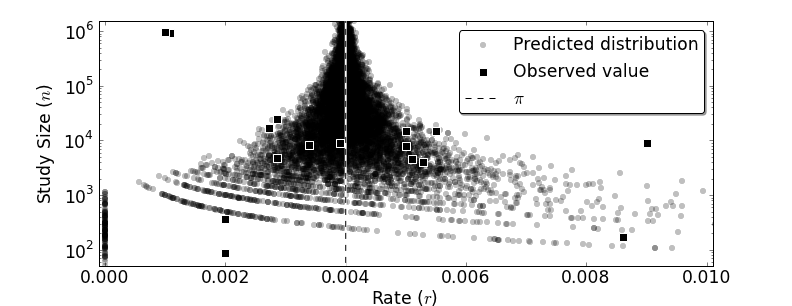
\includegraphics[width=\textwidth]{binomial-model-funnel.png}
\end{center}
\caption{Funnel plot showing predictive distribution for the binomial
  rate model with $\pi=<< rate_model.pi_binomial_funnel >>$ (shown in
  blue), with empirical distribution of TK overlaid for comparison
  (shown in green).}
\label{fig:theory-rate_model-binom_funnel}
\end{figure}

All models are wrong, of course, so why does this model require
refinement? The answer is that is leads to unreasonably high confidence,
which I will now demonstrate.  If a study of $<< rate_model.pop_A_N >>$
 people from in subpopulation A
finds $<< rate_model.pop_A_prev*100 >>\%$ prevalence and a
study of $<< rate_model.pop_A_N >>$ people in subpopulation B
 finds $<< rate_model.pop_B_prev*100
>>\%$ prevalence, then the binomial model predicts that a study of
$<< rate_model.pop_C_N >>$ people in subpopulation C will
 have $<< rate_model.pop_C_prev*100>>\%>>$ prevalence, with $95\%$ HPD interval
$<< rate_model.pop_C_ui >>$.  I have no problem with the point
 estimate.  Picking the mean of the two populations seems just right.
 But the uncertainty interval lacks face validity.  It would be much
 more reasonable to have an uncertainty interval as large as $[5,45]$,
 instead of one as small as this.

One way to formalize this objection is through the posterior predictive
check, an in-sample goodness-of-fit test that can be done
graphically.  Figure~\ref{fig:theory-rate_model-binom_ppc} shows the
posterior predictions of the binomial model when it is fit to the TK
dataset, together with the data itself.  The model predictions are
clearly compressed, and trusting the results of such a model will lead
to inappropriate certainty in the face of noisy data.

\begin{figure}[ht]
\begin{center}
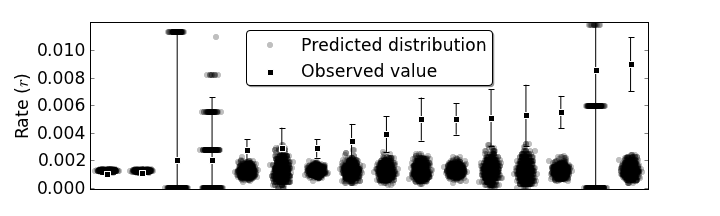
\includegraphics[width=\textwidth]{binomial-model-ppc.png}
\end{center}
\caption{Posterior predictive check for binomial model fit to TK
  data.  Blue shows 1000 draws from the posterior distribution of the
  binomial model, and green shows the input data.}
\label{fig:theory-rate_model-binom_ppc}
\end{figure}




\subsection{Beta-binomial model}
A theoretically appealing extension to the binomial model (which also
does not work for my purposes) is the beta-binomial model.  I will
develop it in this section, to motivate the following sections.

Formally, the beta binomial random variable is given by the following
probability distribution
\begin{align*}
\Pr[X = k|n, \alpha, \beta] 
  &= \int_{\pi}\dens(\pi|\alpha, \beta) \binom{n}{k}\pi^k(1-\pi)^{n-k}
d\pi\\
\dens(\pi|\alpha, \beta) &\propto \pi^{\alpha-1}(1-\pi)^{\beta-1}
\end{align*}

The intuition behind this model is simpler than the equation, however.
Each individual now tests positive for the condition independently
with probability $\pi$ which is itself a random variable, a priori
distributed according to a beta distribution with parameters $\alpha$
and $\beta$. The beta distribution is given by 
\[
\dens(\pi|\alpha, \beta) =
\frac{\Gamma(\alpha+\beta)}{\Gamma(\alpha)\Gamma(\beta)}\pi^{\alpha-1}(1-\pi)^{\beta-1}
\]
and has a high degree of flexibility, as well as the appropriate
support, always taking values between zero and one.
Figure~\ref{fig:theory-rate_model-beta} shows the probability density
of the beta distribution for several combinations of $\alpha$ and
$\beta$.
\begin{figure}[ht]
\begin{center}
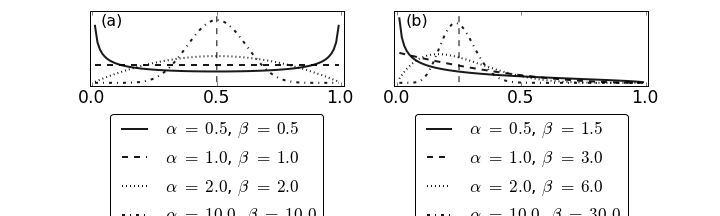
\includegraphics[width=\textwidth]{beta-distribution.png}
\end{center}
\caption{Probability density for the beta distribution for a range of
  $\alpha$ and $\beta$ values. Dashed black line shows expected value,
which is $.5$ for all distribution in a) and $.25$ for all in b).}
\label{fig:theory-rate_model-beta}
\end{figure}

The beta binomial distribution inspired the following rate model for
an observed population rate of $r$ from a population of size $n$:
\[
\dens(r,n|\alpha, \beta) \propto \int_{\pi}
\pi^{\alpha-1}(1-\pi)^{\beta-1} \pi^k (1-\pi)^{n-k}
d\pi.
\]

This model extends the binomial model in a way analogous to how a
random effects model in linear regression.  By introducing an
additional dimension in to the parameter space, it is able to capture
the dispersion beyond the binomial model that I have observed
empirically in funnel plots of real data
(Figure~\ref{fig:theory-rate_beta-binomial-funnel} shows the beta
binomial funnel plot, as well as the posterior predictive check for
this model on the same data as used in
Figure~\ref{fig:theory-rate_model-binom_ppc}.

\begin{figure}[ht]
\begin{center}
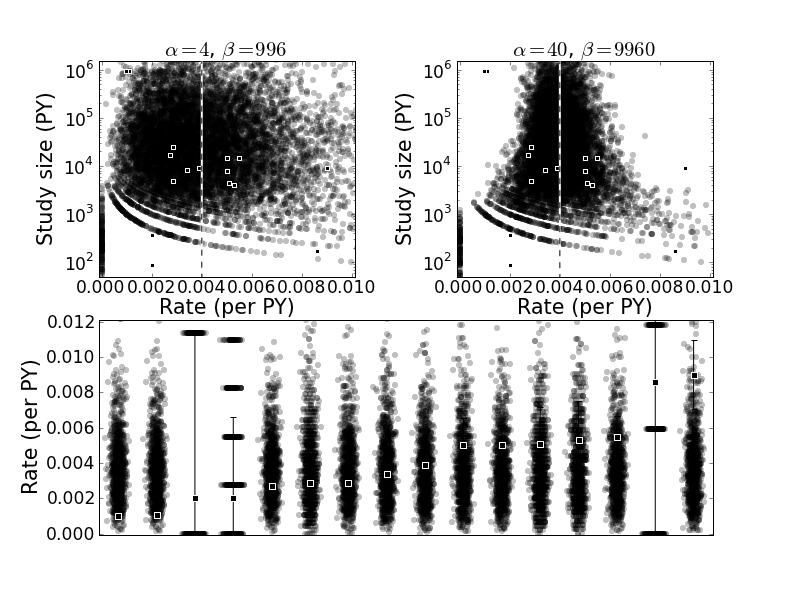
\includegraphics[width=\textwidth]{beta-binomial-funnel.png}
\end{center}
\caption{Funnel plot and posterior predictive check for beta binomial model.}
\label{fig:theory-rate_beta-binomial-funnel}
\end{figure}

This model addresses the theoretical shortcoming raised in the
previous section: if two observations show $1\%$ and $3\%$ prevalence
respectively, the posterior distribution of the beta binomial model
has mean $2\%$ and 95\% HPD interval $[1\%,3\%]$, which seems quite
reasonable.

The great shortcoming of the beta binomial model is computational.  As
will be elaborated in Chapter~\ref{theory-numerical_algorithms}, there
is no closed-form solution to the integral in the probability density
for the beta binomial model.  Evaluating it requires introducing a
latent variable for each of the data points in the likelihood.  This
simply has too much cost for the numerical algorithms and
computational infrastructure available to me currently.  So my search
continues.

\subsection{Approximation to the binomial model}
There are two traditional approximations to the binomial distribution,
depending on how large $k$ is in relation to $n$.  When $k/n$ is
large, the normal distribution is used, and when $k/n$ is small, the
binomial is similar to the Poisson distribution.

Since I expect to usually be in a ``small $k/n$'' setting, I will not
develop the normal model in detail now, although I will return to a
generalization of the normal distribution which subsumes it later.

The Poisson distribution is given by the the equation
\[
\Pr[X=k] = \frac{\lambda^k e^{-\lambda}}{k!},
\]
and it can be understood intuitively as the number of times a
``memoryless'' event occurs in a unit time period.  Setting $\lambda =
\pi n$ produces an approximation to the binomial distribution, which
is quite accurate for large $n$ and small $k$.

TK figure comparing funnel plots and distributions.

The benefit of this alternative is that the over-dispersed variant of
the Poisson distribution, inexplicably called the negative binomial
distribution does have a closed form:
\[
Neg Binom TK,
\]
and exhibits all of the other benefits of the beta binomial
distribution as well.

Closed form

Intuition, RE interpretation, hierarchical description.

A difficultly of the Poisson model and its overdispersed cousin the
negative binomial is in the realm of numerical algorithms.  My
experience has been that these likelihoods lead to models that are
simply harder to fit than traditional normal models.  Nonetheless, the
negative binomial model has been the primary tool in the likelihod
modeling for the applications to be presented in
Chapters~\ref{practice-all-examples}.

\subsection{Alternative Models}

\subsection{Summary and Comparison}
